\documentclass[12pt]{article}
\usepackage{pslatex} % Font Times New Roman

\usepackage{amsmath,amssymb,amsfonts,fancyhdr,lastpage}
\usepackage{makeidx, graphicx}

\setlength{\textheight}{9.0in}
\setlength{\topmargin}{-.5in}
\setlength{\textwidth}{6.5in}
\setlength{\oddsidemargin}{-.0in}
\setlength{\parskip}{6pt}


\renewcommand{\headrulewidth}{0pt}
\setlength{\headsep}{.35in}
\addtolength{\headheight}{2.5pt} 

\usepackage{graphicx}

\begin{document}

\title{Representing Kekule Cells in Stable Molecules}
\author{Aaron Germuth and Alex Aravind \\\\  
Department of Computer Science \\
University of Northern British Columbia \\
E-mail: (germuth,csalex)@unbc.ca}
\maketitle


\begin{abstract}

Certain polycylic polyunsaturated hydrocarbons can preform Boolean operations. Alternating paths of single-double bonds within such molecules have been shown to conduct electricity. 

\end{abstract}

\section{Introduction}

Moore's Law in 1965 \cite{Moore} (not positive about cite here) predicts that, over the history of computing hardware, the number of transistors on a single circuit will double approximately every two years (see Figure 1). Although his prediction has proven to be accurate, there are signs which show this exponential progress is coming to an end \cite{MooreEnd}. Conventional silicon transistors may soon reach their minimum physical size. The amount of leakage current is approaching the order of magnitude of the actual current running through the transistor itself (cite v06[3]).

\begin{figure}[ht!]
\centering
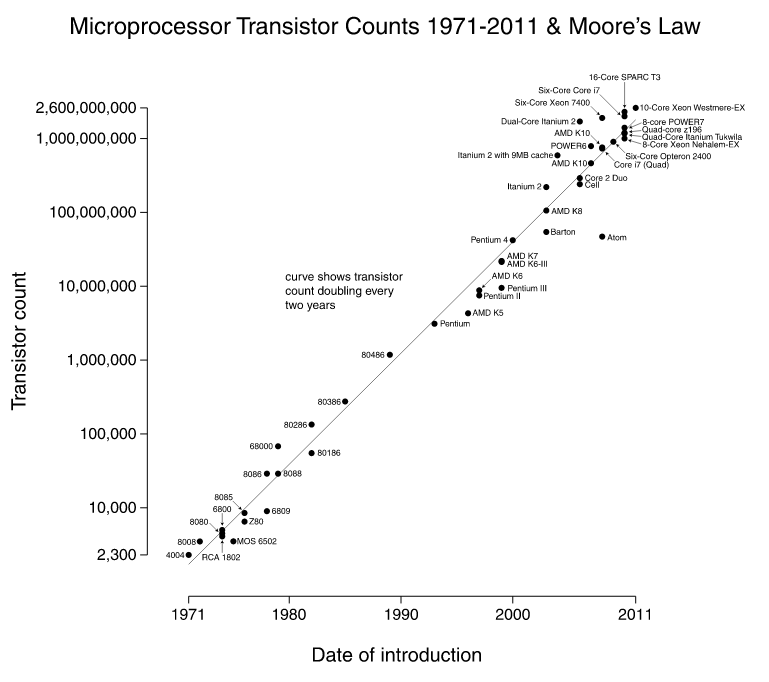
\includegraphics[width=90mm]{MooresLaw.png}
\caption{Plot of CPU transistor counts against dates of introduction, on a logarithmic vertical scale.}
\end{figure}

One alternative possibility to allow smaller circuitry is to use single molecules as computational elements. $\pi$ conjugated organic molecules have been the main focus, and there have been solutions to make them perform as wires \cite{9}, diodes \cite{10,11}, resistors \cite{12,13}, transistors \cite{14, 15, 16, 17}, and switches \cite{18, 19}. Following this it was shown a single molecule can represent an entire Boolean function or logic gate (AND\cite{20} , OR\cite{21}, IF THEN (implication)\cite{22}, NAND\cite{23}, and NOR\cite{24}). Finally, M.H. van der Veen \cite{v06} has shown that a single molecule can facilitate all 16 fundamental logic operations. These molecules can even be combined to achieve bifunctional logic elements with increased complexity.

M. H. van der Veen \cite{v06} not only found a single molecule which has the above characteristics, but then went on to describe $\pi$ logic, a way to determine which Boolean operations any $\pi$ conjugated system can preform. All of this allows for, in theory the design of highly compact and complex logic circuits using $\pi$ conjugated systems. 

In $\pi$ logic, molecules have terminals which consist of atoms where connections outside the molecule can be attached. $\pi$ conjugated wires \cite{9} or omniconjugated molecules \cite{OmniConj} have been suggested to interconnect separate $\pi$ conjugated systems. A pair of terminals is called a pathway. If there exists an alternating single-double bond path from terminal to terminal, the path is deemed 'open'. Open paths have been shown to conduct electricity to a much higher extent than closed paths \cite{openPath}. A path can be alternated (all single bonds become double bonds and vice versa) by sending an electrical 'soliton' over the path \cite{HK88}. A molecule can contain multiple intersecting paths, and in this way, when one path is toggled, another path may be opened or closed (see Figure 2).

\begin{figure}[ht!]
\centering
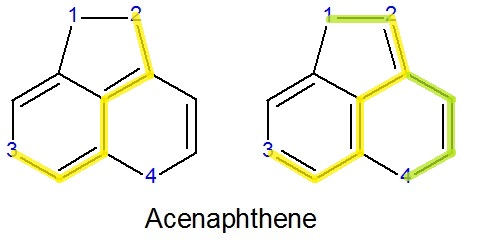
\includegraphics[width=90mm]{AcenaphtheneHighlighted.jpg}
\caption{Acenaphthene displaying switching behavior. There exists an alternating path from terminal 2 to 3 (shown in yellow). When this path is toggled (right diagram), the path from terminal 1 to 4 (shown in green) is also opened.}
\end{figure}

To begin the analysis of a $\pi$ conjugated system using $\pi$ logic, all possible double bond patterns of the molecule are deduced. Two terminals are selected for an output, and whether the path between them is open or closed represents an output of '1' or '0' respectively. The other terminals are paired, and each pair represents an input of '1' or '0', again depending on the openness of the path. From this you can observe all the different Kekul\'e structures of the molecule and map the inputs to the outputs, resulting with a Boolean function. If the terminals are paired in a different orientation, you may redo the process and have the same molecule represent another Boolean function. 

Kekul\'e theory was introduced \cite{HH13} to investigate and systematize this qualitative switching behavior. In Kekul\'e theory, terminals are called ports, and pathways are called channels. A Kekul\'e state is a configuration of bonds such that every node (other than the ports) has precisely one double bond. Ports may or may not have a double bond. Each Kekul\'e state (or resonance structure) of the molecule has a so called port assignment, the set of ports which contain a double bond. A Kekul\'e cell then consists of the set of port assignments for every resonance structure of that molecule (see Figure 3). The rank of a cell or molecule is defined as its number of ports.

\begin{figure}[ht!]
\centering
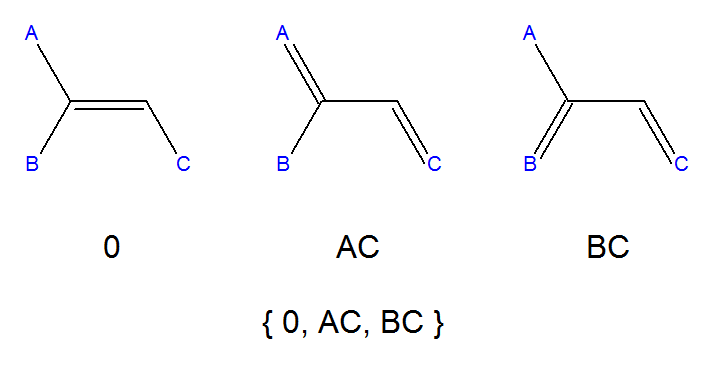
\includegraphics[width=90mm]{KekuleCell.png}
\caption{The Kekul\'e cell of a simple molecule. The 3 structures indicate the 3 possible arrangements of double bonds. The second row indicates the port assignment for each structure, and the third row is the Kekul\'e cell for that molecule. In Hesselink's notation, ports and labeled with letters rather than numbers, and the cell would be \{ 0, ac, bc \} }.
\end{figure}
The switching behavior of a molecule is completely determined by its Kekul\'e cell \cite{HH13, H13}. This allows us to search in the opposite direction from before. Rather than searching for any switching behavior a given molecule may exhibit, we can take a required switching behavior needed in some circuitry element, and then search for a molecule who has this behavior. Hesselink \cite{H13} has developed a method to classify all possible Kekul\'e cells, and has given classifications for all cells with ports \textless 7. Therefore, any switching behavior can be converted to a cell, and any cell can be converted to one of Hesselink's \cite{H13} classified cells.

The next step is to then, given a Kekul\'e cell, find a corresponding molecule which has that cell. In Kekul\'e theory, molecules are abstracted as undirected graphs, where nodes represent atoms, and edges their chemical covalent bonds. These graphs are hydrogen-suppressed as hydrogen plays no role in conjugation. Hesselink \cite{H13} has shown a recursive method which has found graphs for any cell with rank \textless 6 and 210 out of 214 cells with rank 6. 

However, graphs obtained by Hesselink do not represent realistic molecules. In regards to this, Hesselink mentions some methods which can alter a graph without changing it's cell \cite{HH13, v06}. This method however, may be limited for graphs of larger ranks (justification?). We propose an alternative, possibly easier solution for obtaining more realistic graphs. We use a genetic algorithm to create a population of graphs, and evolve them towards their desired Kekul\'e cell. 

\subsection{Overview}

Section 2 consists of the restrictions used to obtain more realistic graphs, and the reasoning behind them. Section 3 explains the genetic algorithm, and how mutation and crossover are applied on graphs. Section 4 presents the results of the genetic algorithms and assesses its validity. This includes how realistic graphs obtained are, and whether these structures can be easily synthesized chemically. Conclusions are drawn in Section 5.

\section{Restrictions}

Carbon is tetravalent, meaning it has 4 valence electrons available to form covalent chemical bonds. This means in most cases, carbon is only stable when bonded with 4 bonding electrons to complete its octet. These 4 electrons may be provided from 4 distinct molecules, or there could be one molecule providing multiple electrons.

In $\pi$ conjugated systems, every carbon atom contains precisely one double bond. Double bonds hold twice the amount of electrons and therefore each carbon can be at most connected to 3 distinct atoms. This is seen in all polycyclic polyunsaturated hydrocarbons. In this way, each node in our graphs has a maximum degree of 3. Ports however, must be able to interact with the outside world. If we assume this connection is through molecular wires, as in \cite{9}, or through an omniconjugated molecule \cite{v06}, then each port must restrict one of it's valence electrons to be able to connect to atoms outside the molecule. For this reason, we restrict ports to have a maximum degree of 2. 

Cycles must also be confined. Due to steric hinderance, cycles such as cyclopropane or cyclobutane are rarely stable in $\pi$ conjugated systems. Huckel's rule states that only cycles with 4n + 2 (2, 6, 10, etc.) delocalized electrons are considered aromatic and stable. However, Huckel's is mainly meant for monocyclic systems, meaning pentagons and heptagons can be stable in certain arrangements (see Azulene, Figure 4). For this reason, we currently only expand cycles of length 3 or 4. 

\begin{figure}[ht!]
\centering
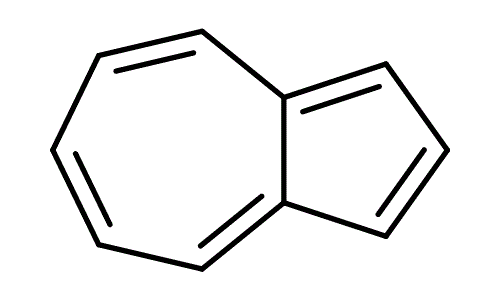
\includegraphics[width=50mm]{azulene.png}
\caption{Azulene, a structure composed of an aromatic heptene and pentene ring attached together.}
\end{figure}

Cycle extension is done by inserting two additional carbon atoms into the cycle at the same position (see Figure 5). This has no effect on the Kekul\'e cell as the two atoms are conjugated with the rest of the ring and simply expand it. This procedure is nearly identical to operation v of \cite{v06}. Care must be taken to not select two nodes which also are a part of another cycle, as the resulting graph will contain unrealistic bonding distances and cycle connectivity. Currently cycles of length 8 and 9 are not reduced to their corresponding cycles of length 6 and 7. 

\begin{figure}[ht!]
\centering
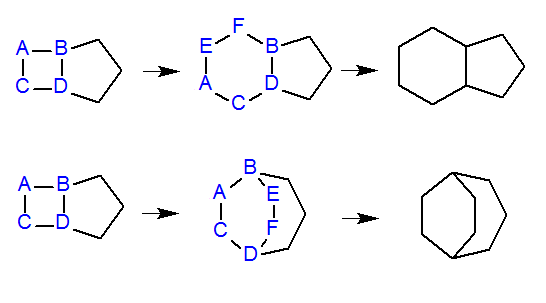
\includegraphics[width=90mm]{cycleExtension.png}
\caption{This shows the extension of the left 4 cycle into a proper 6 cycle. The top half shows a correct procedure when selecting to add two nodes in between A and B. The bottom half shown the incorrect procedure of adding two nodes in between B and D.}
\end{figure}

Cycles are detected using an upper bounded implementation of the 'flooding' algorithm (need cite here). In the flooding algorithm, each node sends out a packet to all if it's neighbors. Any time a node receives a packet, it appends its name and sends the new packet to all of its neighbors. Packets are not sent back to the node who you just received it from. If at any time a packet has been appended by the same node twice, we have found a cycle. As soon as a packet finds a cycle, the packet is discontinued. This process continues to discover all cycles. Packets of length $>$ 12 are also discontinued. This introduces the error that a graph could contain a cycle of length 13. The amount of computation time saved is usually worth it, considering how unlikely a cycle of length 13 or greater is. 

Some optimizations can be made considering the subset of all possible graphs we are dealing with. Packets only begin on nodes with degree of 3, as this is guaranteed to find all cycles (proof?..). If there are no nodes with degree of 3, the graph either contains no cycles, or the graph is one big cycle. Therefore, in this case, we only start a packet at one random node with degree 2. Despite the optimization, this process is still the bottleneck of each iteration for the genetic algorithm.

Not only must cycle size be restricted, but cycle connectivity. In realistic polycyclic polyunsaturated systems, any two rings of the system share at most two nodes. This is seen in naphthalene (see Figure 6), both hexagons share two common atoms. Even in complex polycyclic molecules such as pyracylene (see Figure 6), each cycle shares at most two nodes. Two cycles cannot share a single node (spiro-compound) as the shared node would have a degree of 4. This is why when extending cycles artificially, care must be taken to chose 2 appropriate nodes, as above.

\begin{figure}[ht!]
\centering
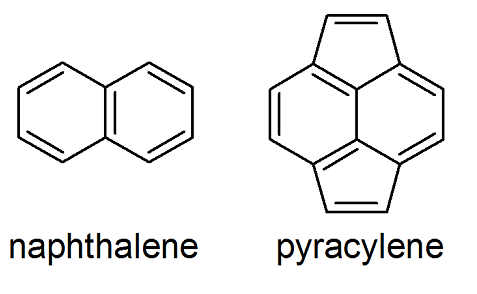
\includegraphics[width=90mm]{polycyclic.png}
\caption{Napthalene shown two benzene rings with 2 carbon atoms is common. Even in complex polycylic hydrocarbons such as pyracylene, every ring shares only 2 carbon atoms.}
\end{figure}

Graphs must be planar. In order for a molecule to be considered aromatic, all of its contributing atoms must be coplanar. This is because aromatic systems are comprised of multiple conjugated bonds. Each $\pi$ conjugated bond results from the overlap in the nodal planes of each bonding atom. This causes a cloud of electron probability above and below the covalent bond. Each cloud generates a small electromagnetic field, which works to keep the ring flat (need cite here). A consequence of planarity is that any graph of the molecule should be able to visualized such that no edges are intersecting. (  currently we don't detect whether graphs are planar or not ) 

Finally, graphs representing molecules must be connected. A disjoint graph represents two molecules rather than one. Two disjoint graphs can sometimes be connected using the following procedure. If we add internal vertices which must always conjugate ’within’ themselves, they will not interfere with the cell. For example, see Figure X (PICTURE).

include figure X here

Figure 2: Transforming a disjoint graph into a connected one. Ports are represented by encircled nodes.

In the right-hand graph of Figure 2, y is not a port and so must always contain a double bond. The only other node which is available to form a double bond with y is x, so in every resonance structure of this molecule x and y will contain a double bond with each other. Therefore d or b can never form a double bond with their new edge, and the Kekul\'e cell has not been changed. This now resembles a stable connected molecule.
This procedure is similar to Operation iii and Operation vi of [3].

Although these restrictions do a good job of trimming out almost all unrealistic graphs, they are not absolute. Cycles of length 5 and 7 are seen in naturally occurring hydrocarbons, but it is difficult to determine what arrangement makes than stable (need more research here). Additionally, our procedure makes no attempt to ensure all bonding distances are realistic (PICTURE)(which can occur when cycles above the limit are perceived) and the molecules displayed can be synthesized. 

\section{Genetic Algorithm}

A genetic algorithm is used to search for graphs which apply to a given cell. The algorithm begins by randomly generating a population of graphs. Each starting graph has anywhere from rank to 31 nodes, and rank - 1 to 20 edges. There must be at least rank - 1 edges in order to connect the the minimum amount of nodes together. Graphs with fitness 0 or lower (normally arises from disconnected ports) are deleted and a new graph will take its place. This makes up the first generation.

In each iteration, the survivors of last generation's population must be chosen. This is done by selecting the best preforming graphs (fitness-wise), along with a smaller amount of random graphs. Random graphs are added to ensure genetic diversity in the population. This sub-population of now undergoes genetic operations such as mutation and crossover. 

The genetic algorithm has two terminating conditions. Either the maximum number of iterations has been reached, or some threshold of graphs which satisfy the cell has been reached. In some smaller cases, the genetic algorithm terminates immediately after generating the initial population, as it contained at least x graphs which satisfy the cell ( where x is the threshold of graphs desired).

If no graphs are found which satisfy the cell and the restrictions of Section 2, it is possible the genetic algorithm will display graphs who satisfy the cell, but do not satisfy all restrictions. Not sure if we want this. Need to explain why fitness decremented instead of removed for bad graphs. IS this even what we want.

Resulting graphs are converted to SMILES (small molecular input line entry system) in order to be visualized. Conversion first involves finding a spanning tree of the graph. All edges in the original graph which are not in the spanning tree must be edges which complete a cycle. Therefore each node on either side of the edge is labeled as a cycle point. We then preform depth first search over the spanning tree, and append each nodes label as we reach it.

The ports are labeled by atoms with a P (normally reserved for phosphorous, but we can ignore this here). The open source Chemistry Development Kit (cite) is then used to parse the SMILES and generate a 2D structure. Other than the ports, the structure resembles the hydrogen-suppressed carbon skeleton of the structure.  

\subsection{Mutation}

Mutation involves randomly perturbing graphs to obtain new ones. We normally  generate enough mutants so that it is likely each graph will be mutated more than once. Mutations include:
\begin{enumerate}
\item 20 \% chance to add a new node
\item 20 \%  chance to remove a random node, and all edges to it
\item 40 \% chance to add a random edge \footnote{ Edges are randomly chosen until an edge is found that can be added without breaking our restrictions on the degree of vertices.}
\item 40 \% chance to remove a random edge
\end{enumerate}

\subsection{Crossover}

Crossover begins by randomly selecting 2 graphs from the sub-population. These graphs are combined to create a new child graph. On average, each graph produces two children. Children receive all edges with both parents share, and have a 50\% chance to get any other edge found in one of the parents. This creates children which are a hybrid of both their parents.

\subsection{Fitness Function}

Fitness values are integers given to a graph. Any graphs cell can be calculated using Hesselink's procedure here: (explain a lot ). The fitness is calculated by iterating over the graphs cell compared to the cell we are evolving towards. For every port assignment they share, the fitness is incremented by one. For every port assignment that is missing, or is extra, fitness is decremented one point. If a cell is empty, with no port assignments \footnote{This can happen when the genetic algorithm creates a graph which has a (non-port) vertex with no edges to it (degree 0). There is no way for this graph to have a Kekul\'e structure since the lone vertex can never have a double bond.}, it is given a fitness value of -10, in attempt to discourage that graph from evolving onward. 

\subsection{Additional Note}

It should be noted that rather than using the genetic algorithm to approximate a solution (as seen in most applications), an answer generated by it is only useful if it found an actual solution. However, for all cells of rank \textless 6 and most cells of rank 6, the genetic algorithm can converge to multiple solutions for a given cell. 

\section{Results}

Ask Alex about blatantly copying citations.

\section{Conclusion}


\begin{thebibliography}{abrv}

\bibitem{H13} W. H. Hesselink, Graph Theory for alternating hydrocarbons with attached ports. Indagationes Mathematicae, Elsevier, 24:115141, 2013.
\bibitem{HH13} W.H. Hesselink, J.C. Hummelen, H.T. Jonkman, H.G. Reker, G.R. Renardel de Lavalette, M.H. van der Veen, Kekule Cells for Molecular Computation. Cornell University Library Online, 2013.
\bibitem{v06} M.H. van der Veen. $\pi$-Logic. PhD thesis, University of Groningen, May 2006.
\bibitem{HK88} A.J. Heeger, S. Kivelson, J.R. Schrieffer, and W.-P Su. Solitons in conducting polymers, Rev. Mod. Phys.,60:781, 1988.
\bibitem{Moore} G. E. Moore, Cramming more components onto integrated circuits. Electronics Magazine. p. 4. Retrieved 2006-11-11. 
\bibitem{MooreEnd} C. A. Mack, Fifty Years of Moore's Law. IEEE Transactions on semiconductor manufacturing, 24:2 2011.
\bibitem{OmniConj} M. H. van der Veen, M. T. Rispens, H. T. Jonkman, and J. C. Hummelen, Molecules with Linear $\pi$-Conjugated Pathways between all Substituents: Omniconjugation. Adv. Function Mater, 14:3, 2004.
\bibitem{openPath} S.N. Yalirahi, M.A. Ratner, Interplay of topology and chemical stability on the electronic transport of molecular junctions, Ann. New York Acad. Sci. 960 (2002) 153.
\bibitem{9} J. Reichert, R. Ochs, D. Beckmann, H. B. Weber, M. Mayor, H. von Löhneysen,Phys. Rev. Lett. 2002, 88, 176804. 
\bibitem{10} A. Aviram, M. A. Ratner, Chem. Phys. Lett. 1974, 29, 277.
\bibitem{11} D. B. Strukov, K. K. Likharev, Nanotechnology 2005, 16, 137.
\bibitem{12} Y. Karzazi, J. Cornil, J. L. Brédas, J. Am. Chem. Soc. 2001, 123, 10076.
\bibitem{13} J. M. Tour, M. Kozaki, J. M. Seminario, J. Am. Chem. Soc. 1998, 120, 8486.
\bibitem{14} A. Aviram, J. Am. Chem. Soc. 1988, 110, 5687.
\bibitem{15} H. W. Ch. Postma, T. Teepen, Z. Yao, M. Grifoni, C. Dekker, Science 2001, 293, 76.
\bibitem{16} C. Joachim, J. K. Gimzewski, Chem. Phys. Lett. 1997, 265, 353.
\bibitem{17} T. D. Anthopoulos, C. Tanase, S. Setayesh, E. J. Meijer, J. C. Hummelen, P. W. M. Blom, D. M. de Leeuw, Adv. Funct. Mater. 2004, 16, 2174.
\bibitem{18} G. M. Tsivgoulis, J.-M. Lehn, Chem. Eur. J. 1996, 2, 1399.
\bibitem{19} J. J. D. de Jong, L. N. Lucas, R. M. Kellogg, J. H. van Esch, B. L. Feringa, Science 2004, 304, 278.
\bibitem{20} A. P. de Silva, H. Q. N. Gunaratne, C. P. McCoy, Nature 1993, 364, 42.
\bibitem{21} F. M. Raymo, S. Giordani, J. Org. Chem. 2003, 68, 4158.
\bibitem{22} K. Rurack, A. Koval'chuck, J. L. Bricks, J. L. Slominskii, J. Am. Chem. Soc. 2001, 123, 6205.
\bibitem{23} D. Parker, J. A. G. Williams, Chem. Commun. 1998, 245.
\bibitem{24} A. P. de Silva, I. M. Dixon, H. Q. N. Gunaratne, T. Gunnlaugsson, P. R. S. Maxwell, T. E. Rice, J. Am. Chem. Soc. 1999, 121, 1393.

\end{thebibliography}

\end{document}
